\chapter{Part I(e) - ISA Arithmetic - W 3.1}
\section{Notation}
Before we start, let's define some notation:
\begin{itemize}
    \item[-] \textbf{Number representation (with a fixed number of digits/bits):}
    \[
    A = A^{(n)} = A^{(m)}
    \]
    
    \item[-] \textbf{Number in binary or decimal:}
    \[
    A = A_{10} = A_{2} = A_{2c}
    \]
    \textit{With $A_{2c}$ being the 2's complement representation.} \\
    \textit{And $A_{2}$ being the binary representation.}
    \item[-] \textbf{Individual digits or bits:}
    \[
    a_{n-1}, a_{n-2}, \dots, a_2, a_1, a_0
    \]
    
    \item[-] \textbf{Digit string representation:}
    \[
    \langle a_{n-1} a_{n-2} \dots a_2 a_1 a_0 \rangle
    \]
\end{itemize}

\section{Numbers}

Numbers in computing can be represented in different forms, each with specific use cases. \\
\vspace*{5px}
\textbf{Integers} can be either signed or unsigned, representing positive and negative values, or only non-negative values. Examples include:
\[
0, 1, 2, 3, 4294967295, -2147483648
\]

\textbf{Fixed-point} numbers are essentially integers with an implicit scaling factor (e.g., \(10^k\) or \(2^k\)) to handle fractional values. Common in applications like signal processing. Examples include:
\[
0.12, 3.14, 1073741823.75
\]

\textbf{Floating-point} numbers represent a wide range of values using a base and exponent, providing flexibility in precision. Examples include:
\[
3.14E3, -2.5E1, 1.0E0, 4.2E-2, -1.5E-3
\]

\subsection{Unsigned Integers}
Unsigned integers are:
\begin{itemize}
    \item[-] \textit{Weighted}: Each digit has a positional value.
    \item[-] \textit{Nonredundant}: Every number has a unique representation.
    \item[-] \textit{Based on a fixed-radix system}: Typically radix-10 (decimal) or radix-2 (binary).
    \item[-] \textit{Canonical}: Follows a standard form for representation.
\end{itemize}

\textbf{Definition:}
\[
A = \langle a_{n-1} a_{n-2} \dots a_2 a_1 a_0 \rangle = \sum_{i=0}^{n-1} a_i R^i
\]
where \(A\) is the unsigned integer, \(a_i\) are the digits, and \(R\) is the radix.

\subsection{Signed Integers}
We may distinguish between three methods for representing signed integers:
\begin{itemize}
    \item \textbf{Sign-and-Magnitude (SM)}: Uses the most significant bit (MSB) to represent the sign (0 for positive, 1 for negative), with the remaining bits representing the magnitude. This method has the drawback of two zeros (+0 and -0) (Redundant).
    \item \textbf{Two's Complement}(Specific True-and-Complement): The most common way to represent signed integers. It avoids the two-zero problem and simplifies arithmetic operations. Negative numbers are represented by flipping the bits and adding 1.
    \item \textbf{Biased Representation}: Primarily used in floating-point numbers, especially for the exponent part. A fixed bias is added to the actual value to avoid negative exponents. It's rarely used for integers but is another method for handling signed numbers.
\end{itemize}
\subsubsection{Sign and Magnitude}
In the sign-and-magnitude representation, the most significant bit (MSB) is used to represent the sign of the number. The remaining bits represent the magnitude. \\
\vspace*{7px}
\textbf{Definition} \\
\vspace*{3px}
\[
A = \langle s a_{n-2} a_{n-3} \dots a_2 a_1 a_0 \rangle = (-1)^s \cdot \sum_{i=0}^{n-1} a_i R^i
\]
where \(A\) is the signed integer, \(s\) the most significant bit of \(A\) representing the sign of the number, \(a_i\) the digits, and \(R\) the radix. \\
\vspace*{7px}
\textbf{Example (Signed 4-bit integer):} \\
\vspace*{3px}

Consider the 4-bit signed binary number \(1011_2\). In this case: \\
\begin{itemize}
    \item[1.] The MSB \(s = 1\), indicating the number is negative.
    \item[2.] The magnitude bits are \(011_2 = 3_{10}\).
    \item[3.] Therefore, the value of the number is \(-3\).
\end{itemize}

Thus, \(1011_2\) represents \(-3_{10}\) in sign-and-magnitude representation. \\
\vspace*{7px}

\subsection{Radix's Complement}
Radix's complement is a method used to represent signed numbers in different number systems. \\
It is a special form of \textit{true-and-complement} where the complement $C = R^n$, with $R$ being the radix (base) and $n$ the number of digits. \\
\vspace*{5px}
\begin{center}
    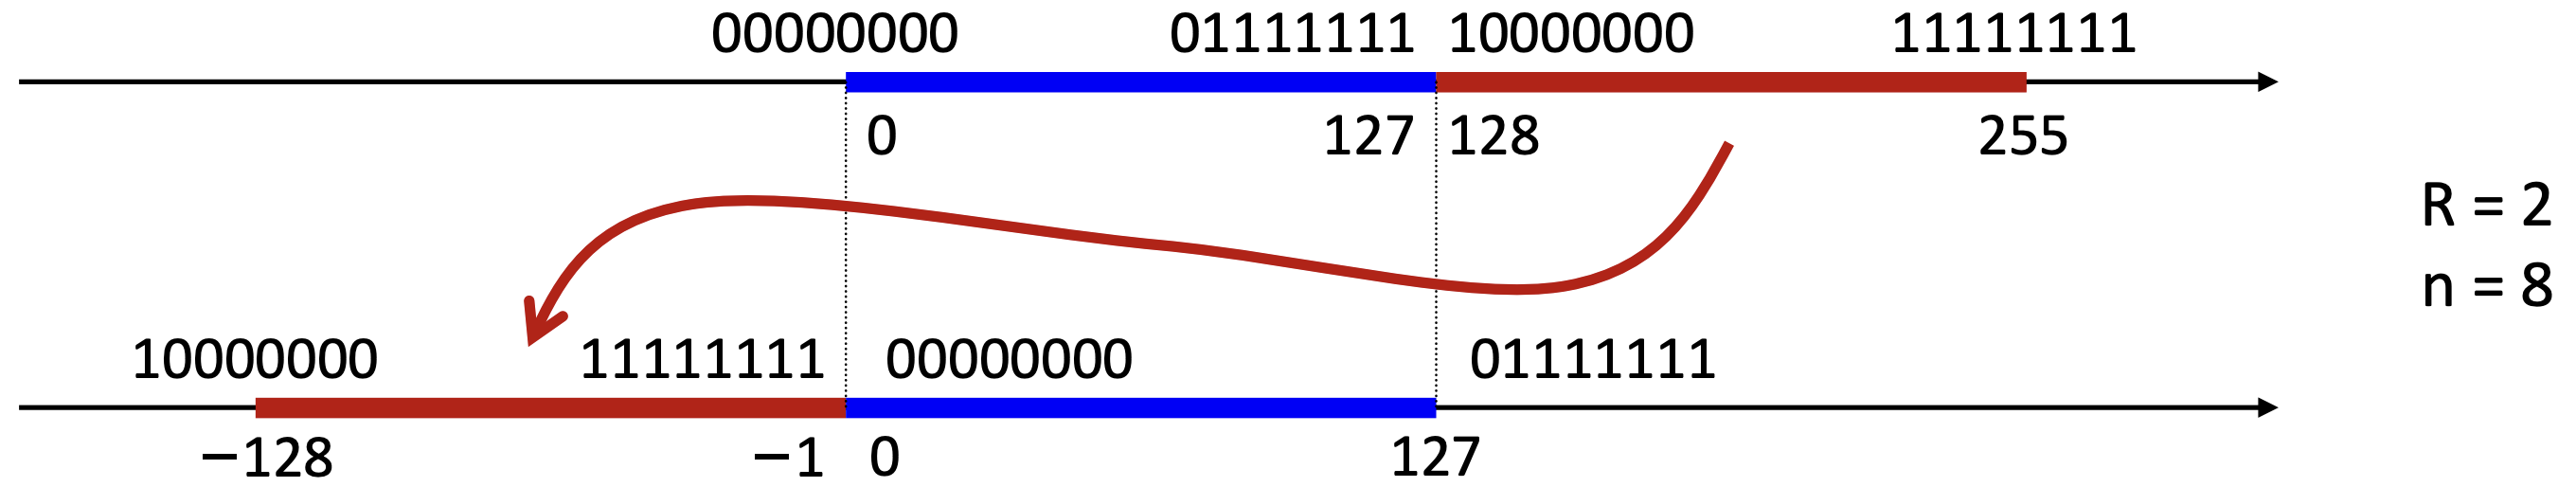
\includegraphics[width=0.65\textwidth]{chapters/chapter1e/images/twoscomplement.png}
\end{center}
\textbf{Definition} \\
\vspace*{2px}
A number $A$ in radix's complement is represented as:
\[
A = \langle a_{n-1}a_{n-2}\dots a_1a_0 \rangle = -a_{n-1}R^{n-1} + \sum_{i=0}^{n-2} a_i R^i
\]
where $a_{n-1}$ is the most significant bit, which also indicates the sign (negative for $a_{n-1} = 1$). \\
\vspace*{5px}
For binary numbers, radix’s complement is known as \textbf{two's complement}, which is the most commonly used method for representing signed numbers in digital systems. \\
\vspace*{5px}
\textbf{Binary (2's Complement) Representation} \\
\vspace*{2px}
Two's complement uses base $R = 2$ and has a fixed word length $n$. \\
Here is an example for an 8-bit number system:



\begin{center}
\begin{tabular}{|c|c|c|}
\hline
\textbf{Binary} & \textbf{Decimal} & \textbf{Range} \\
\hline
00000000 & 0   & \multirow{2}{*}{Positive range} \\
01111111 & 127 & \\
\hline
10000000 & -128 & \multirow{2}{*}{Negative range} \\
11111111 & -1   & \\
\hline
\end{tabular}
\end{center}

The two's complement system enables representation of both positive and negative numbers within a fixed bit length. \\
\vspace*{5px}
\textbf{Decimal (10's Complement) Representation} \\
\vspace*{2px}
In a decimal system with radix $R = 10$,\\
We use 10's complement to represent signed numbers. For instance: \\
\[
5,678_{(5)}^{10c} = 05,678_{10c} = +5,678_{10}
\]
This is a positive number representation in 10's complement. For a negative number: \\

\[
9,999,999_{(7)}^{10c} = -1_{10}
\]
Here, $9,999,999$ in 7 digits represents $-1$ in decimal form. \\
\vspace*{5px}
\textbf{Examples of Binary (2's Complement)} \\
\vspace*{2px}
Below are several examples of numbers in binary (2's complement) and their corresponding decimal values: \\
This is a positive binary number. \\
\[
0100,1101,0010_{(12)}^{2c} = 100,1101,0010_2 = +1,234_{10}
\]

This is a negative binary number in 8-bit representation.\\
\[
1111,1111_{(8)}^{2c} = -1_{10}
\]

This is a negative binary number in 12-bit representation.\\
\[
1011,0000,1110_{(12)}^{2c} = -1,234_{10}
\]
\vspace*{5px}

\subsection{Two's Complement Subtraction}

Consider the binary subtraction using the standard paper-and-pencil method:

\[
\begin{array}{cccccccccc}
\text{Borrow:} & -1 & -1 & -1 & & & & -1 & & \\
& 0 & 0 & 0 & 0 & 1 & 0 & 1 & 0 & \quad (10_{10}) \\
- & 0 & 0 & 0 & 1 & 0 & 0 & 0 & 1 & \quad (17_{10}) \\
\hline
  & 1 & 1 & 1 & 1 & 1 & 0 & 0 & 1 \\
\end{array}
\]


Since we had to borrow beyond the most significant bit, the result is negative. The binary result is:
\[
-1\ 1\ 1\ 1\ 1\ 0\ 0\ 1_2
\]

To find its decimal value:
\begin{center}
    $-2^7 + 2^6 + 2^5 + 2^4 + 2^3 + 2^0 = -128 + 64 + 32 + 16 + 8 + 1 =-7$ \\
    and \\
    $
    10_{10} - 17_{10} = -7_{10}
    $
\end{center}


\subsection{Addition Is Unchanged from Unsigned}

In arithmetic operations, addition remains consistent whether using signed or unsigned numbers. The following instructions are available for basic arithmetic operations:
\begin{center}
    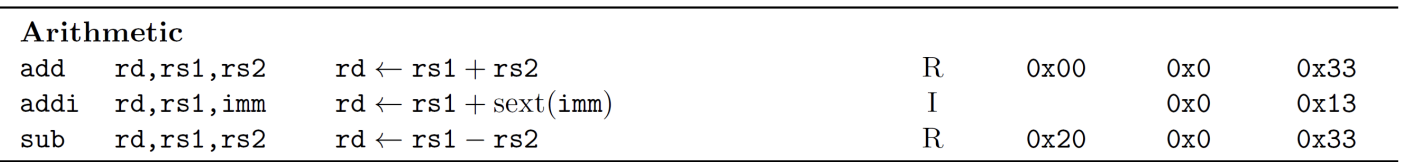
\includegraphics[width=0.75\textwidth]{chapters/chapter1e/images/addition.png}
\end{center}
\begin{itemize}
    \item[-] \texttt{add rd, rs1, rs2}: Adds the values in \texttt{rs1} and \texttt{rs2}, and stores the result in \texttt{rd}.
    \item[-] \texttt{addi rd, rs1, imm}: Adds the value in \texttt{rs1} with the sign-extended immediate value \texttt{imm}, and stores the result in \texttt{rd}.
    \item[-] \texttt{sub rd, rs1, rs2}: Subtracts the value in \texttt{rs2} from \texttt{rs1}, and stores the result in \texttt{rd}.
\end{itemize}
 
Note that older architectures (e.g., MIPS) had distinct instructions for signed (\texttt{add}) and unsigned (\texttt{addu}) addition. However, this distinction is unnecessary as the hardware handles both identically. \\
\vspace*{5px}
Sign-and-magnitude addition presents unique challenges, making \textbf{two's complement} the standard for signed integers in modern architectures.

\subsection{Sign Extension}

In digital systems, sign extension is a technique used to increase the bit width of a binary number while preserving its value and sign. It is commonly used when converting a number from a smaller to a larger bit width in a way that maintains its original meaning, whether it's unsigned or in two’s complement format.


\subsubsection{Example: 4-bit to 8-bit Conversion}
Consider the 4-bit two’s complement number \( 1110_2 \), which represents \( -2_{10} \).\\
When extending this number to 8 bits, we replicate the MSB (which is 1 in this case) to fill the additional bits, as shown below: \\
\[
5_{10} = 0101_2 \quad \text{(4 bits)} \to \quad 00000101_2 \quad \text{(8 bits)}.
\] \\
while 
\[
-2_{10} = 1110_2 \quad \text{(4 bits)} \quad \to \quad 11111110_2 \quad \text{(8 bits)}.
\]

This ensures that the number remains \( -2_{10} \) even after increasing the bit width. \\
\vspace*{5px}


\textit{\textbf{Truncation} is allowed when reducing bit width, but only if the truncated bits are redundant (i.e., copies of the sign bit). For example, going from 8 bits back to 4 bits would result in \( 1110_2 \), preserving the value \( -2_{10} \).
}

\subsection{Signed and Unsigned Instructions}
In RISC-V, instructions differentiate between signed (s) and unsigned (u) operations:

\begin{center}
    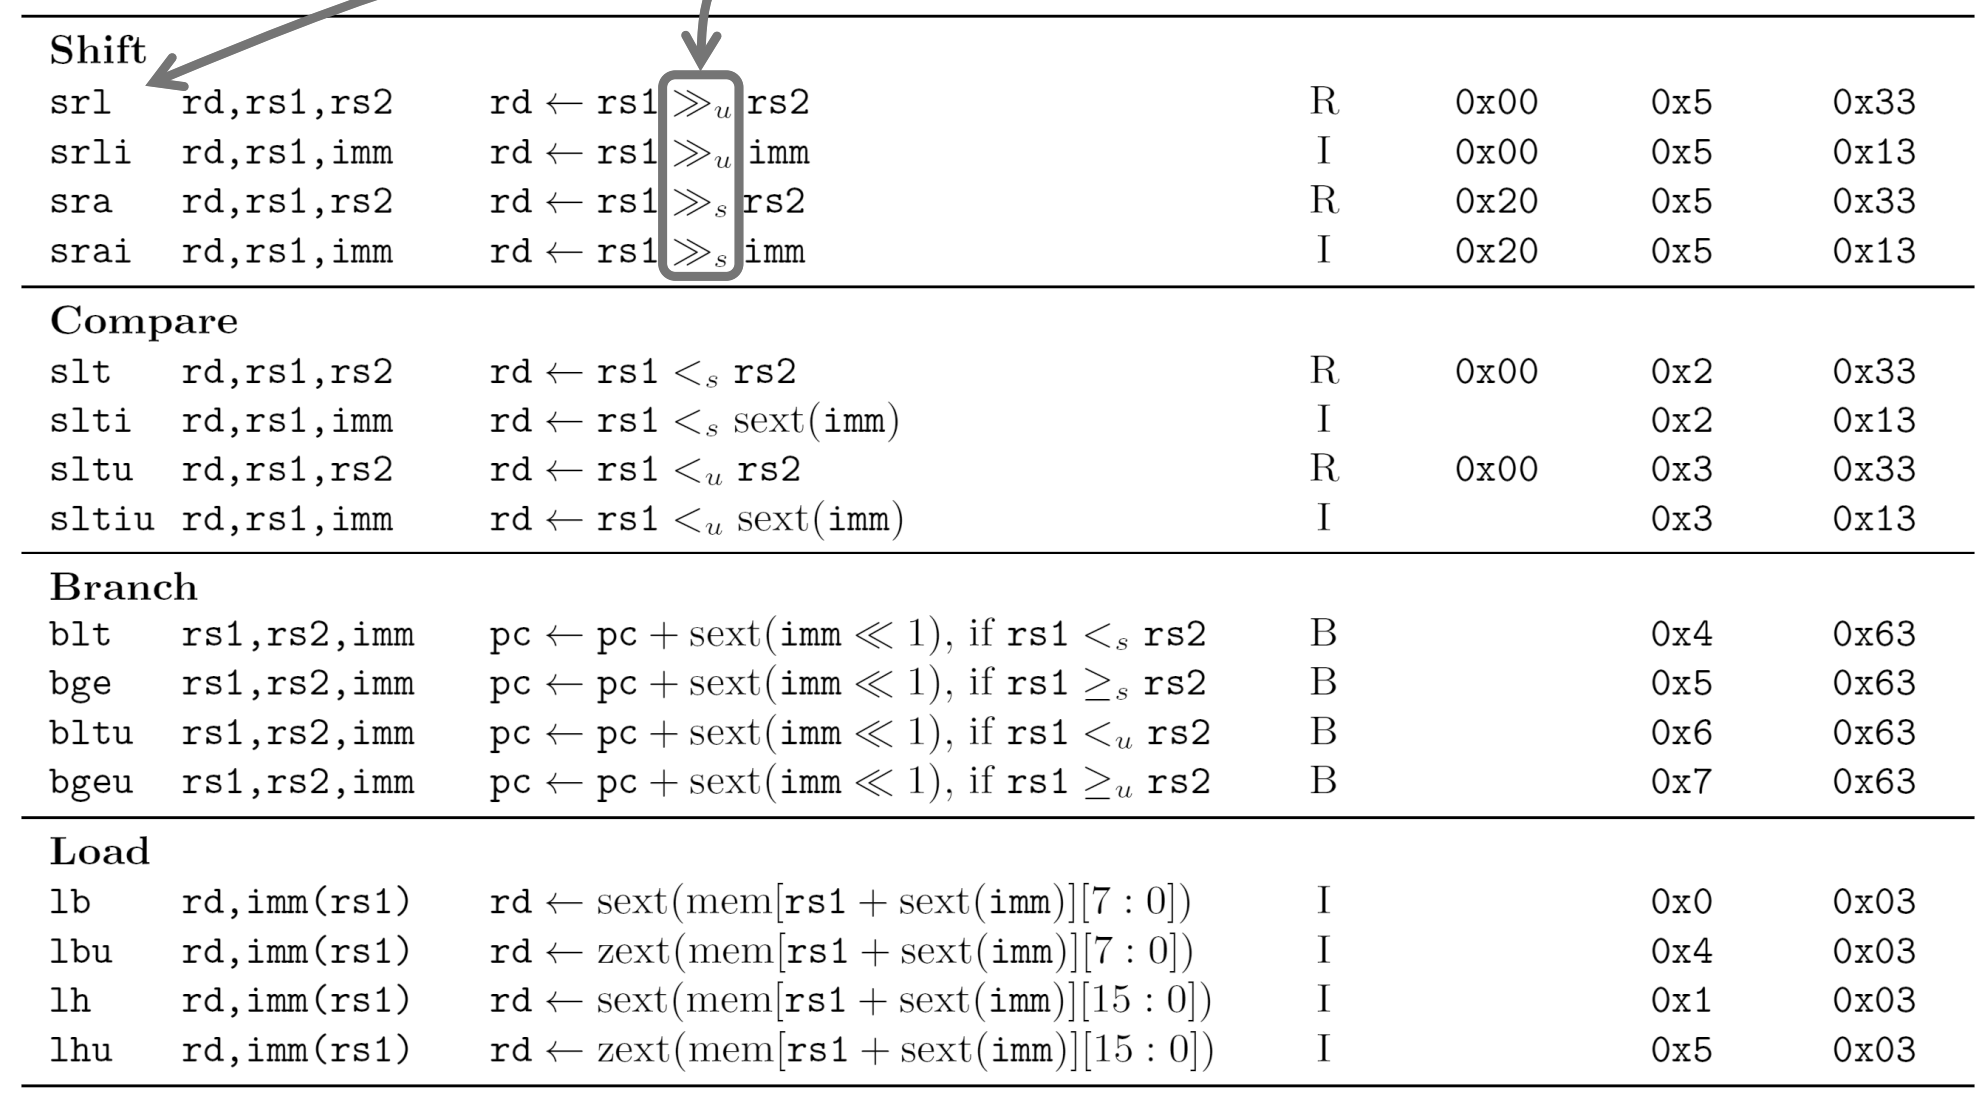
\includegraphics[width=0.75\textwidth]{chapters/chapter1e/images/ref_card.png}
\end{center}
\begin{itemize}
    \item \textbf{Shift:} \texttt{sra}, \texttt{srai} (s) vs. \texttt{srl}, \texttt{srli} (u). 
    \begin{itemize}
        \item Signed shifts preserve the sign bit, while unsigned shifts insert zeroes.
    \end{itemize}
    
    \item \textbf{Compare:} \texttt{slt}, \texttt{slti} (s) vs. \texttt{sltu}, \texttt{sltiu} (u). 
    \begin{itemize}
        \item Signed comparisons use two's complement, unsigned comparisons ignore sign.
    \end{itemize}
    
    \item \textbf{Branch:} \texttt{blt}, \texttt{bge} (s) vs. \texttt{bltu}, \texttt{bgeu} (u). 
    \begin{itemize}
        \item Signed branches use two's complement; unsigned branches do not consider sign.
    \end{itemize}
    
    \item \textbf{Load:} \texttt{lb}, \texttt{lh} (s) vs. \texttt{lbu}, \texttt{lhu} (u). 
    \begin{itemize}
        \item Signed loads extend the sign bit, while unsigned loads extend with zeroes.
    \end{itemize}
\end{itemize}


\section{Overflow}

Overflow occurs when the result of an arithmetic operation exceeds the range of values that can be represented with a fixed number of bits. This can happen in both unsigned and signed arithmetic, though the detection method differs. In general, overflow results in an incorrect outcome that needs to be detected and handled.

\subsection{Overflow in 2's Complement}

In 2's complement arithmetic, overflow occurs when the result of an addition or subtraction operation falls outside the representable range for the number of bits. For an \(n\)-bit 2's complement system, the representable range is \(-2^{n-1}\) to \(2^{n-1} - 1\).

Overflow is detected by examining the carry into and out of the most significant bit (MSB). Specifically, overflow occurs if:

\[
\text{Overflow} = \text{Cout}_{n-1} \oplus \text{Cout}_n
\]

Where:
\begin{itemize}
    \item[-] \(\text{Cout}_{n-1}\) is the carry into the MSB.
    \item[-] \(\text{Cout}_n\) is the carry out of the MSB.
\end{itemize}

An overflow occurs when these two carry bits differ. This is because the sign of the result is incorrect if there is a mismatch, leading to an incorrect outcome.

\begin{center}
    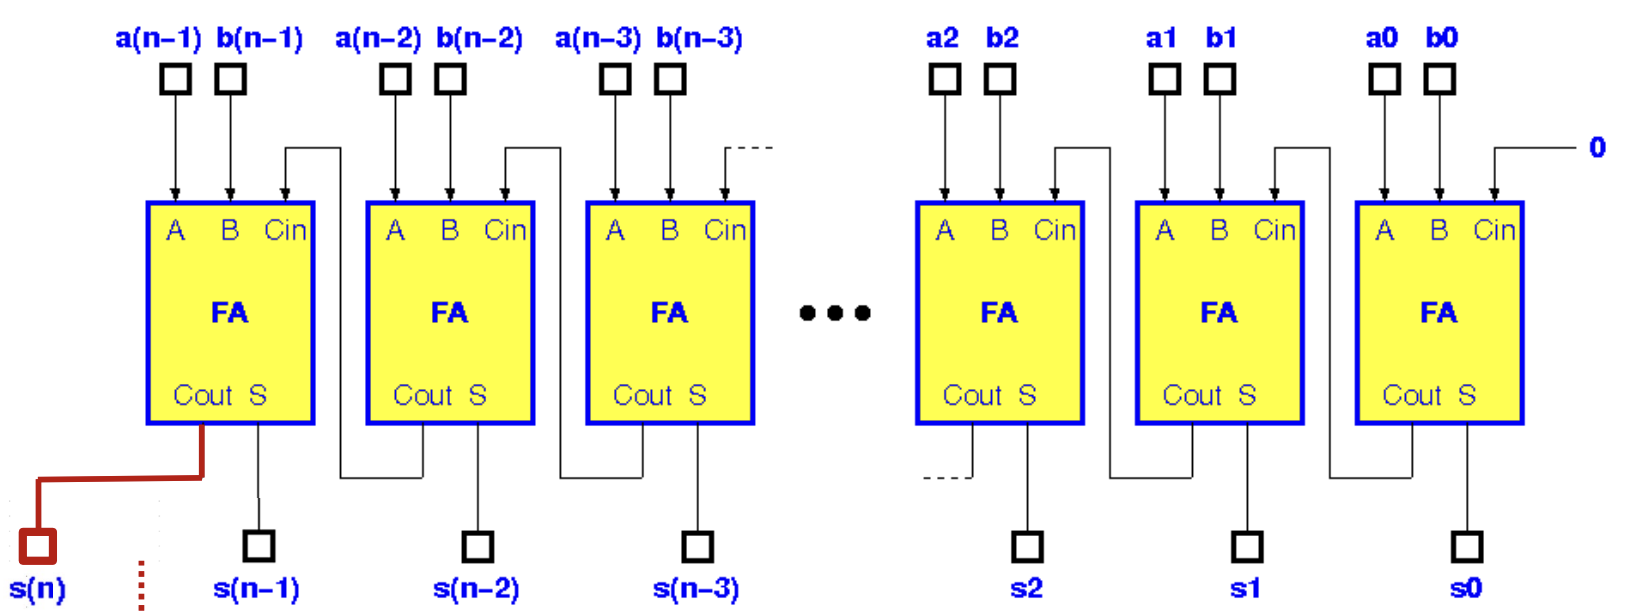
\includegraphics[width=0.65\textwidth]{chapters/chapter1e/images/sum.png}
\end{center}

For example, if two large positive numbers are added and result in a negative value (or two negative numbers added result in a positive value), this indicates an overflow in 2's complement addition.

\subsection{Overflow in Software}

In many architectures, detecting overflow during arithmetic operations is a critical aspect of software implementation. Overflow occurs when the result of an addition or subtraction exceeds the capacity of the register used to store it. Detection methods vary depending on the type of architecture:

\begin{itemize}
    \item \textbf{Traditional architectures (e.g., x86):} These systems provide a \textit{carry bit} in a special register, known as a flag, that is set when an overflow occurs. Thus, overflow detection operates similarly to hardware-based overflow detection.
    
    \item \textbf{Modern architectures (e.g., RISC-V):} These architectures typically provide only the result of the addition or subtraction without a carry bit. Overflow detection must be handled in software, based on analyzing the sign and magnitude of the result.
\end{itemize}

\begin{center}
    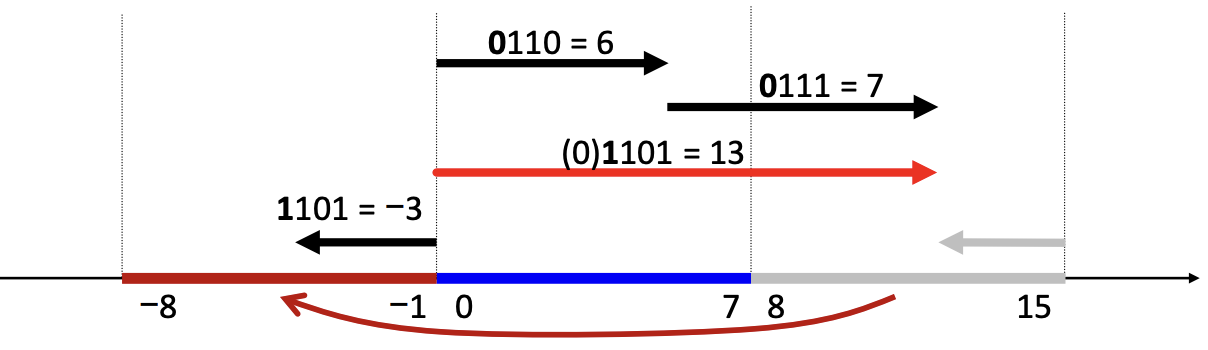
\includegraphics[width=0.65\textwidth]{chapters/chapter1e/images/overflow.png}
\end{center}
Overflow detection can be based on the following observations:
\begin{itemize}
    \item[-] \textbf{Addition of opposite sign numbers:} The magnitude of the result decreases, making overflow impossible.
    \item[-] \textbf{Addition of same sign numbers:} Overflow is possible if the result exceeds the range representable by the register, leading to an incorrect sign in the result.
\end{itemize}
\subsection{Detect Addition Overflow in Software}
\begin{itemize}
    \item[-] Add two 32-bit signed integers and detect overflow
    \begin{itemize}
        \item At call time, a0 and a1 contain the two integers
        \item On return, a0 contains the result and a1 must be nonzero in case of overflow
    \end{itemize}
\end{itemize}


\subsection{Detect Addition Overflow in Software}
\begin{itemize}
    \item[-] Add two 32-bit signed integers and detect overflow
    \begin{itemize}
        \item At call time, \texttt{a0} and \texttt{a1} contain the two integers.
        \item On return, \texttt{a0} contains the result and \texttt{a1} must be nonzero in case of overflow.
    \end{itemize}
\end{itemize}

\begin{assembly}
srai a2, a0, 31       # a2 = sign of a0 (0 or -1)
srai a3, a1, 31       # a3 = sign of a1 (0 or -1)
xor  a4, a2, a3       # a4 = 0 if signs are same, -1 if different
add  a0, a0, a1       # compute sum in a0
srai a5, a0, 31       # a5 = sign of sum (0 or -1)
xor  a6, a2, a5       # a6 = 0 if sign of sum same as a0, -1 if different
and  a1, a4, a6       # a1 = -1 if overflow occurred, else 0
srli a1, a1, 31       # a1 = 1 if overflow occurred, else 0
\end{assembly}

\section{A Strange but Useful Property}
\textit{Personal Remark: don't mistake A and $\overline{A}$ as sets of elements which might confuse you. They are binary numbers.} \\
In binary arithmetic, there is a particularly useful property that can be expressed as follows:

\[
A + \overline{A} = -1
\]
or equivalently,
\[
-A = \overline{A} + 1
\]

\textbf{Proof:} Consider a binary number $A = a_{n-1}2^{n-1} + \sum_{i=0}^{n-2} a_i 2^i$, where $a_i \in \{0,1\}$ represents the binary digits of $A$. The complement of $A$, denoted $\overline{A}$, is given by replacing each $a_i$ with its complement $\overline{a_i}$.

\[
A + \overline{A} = \left( -a_{n-1}2^{n-1} + \sum_{i=0}^{n-2} a_i 2^i \right) + \left( -\overline{a_{n-1}} 2^{n-1} + \sum_{i=0}^{n-2} \overline{a_i} 2^i \right)
\]
\[
= -(a_{n-1} + \overline{a_{n-1}}) \cdot 2^{n-1} + \sum_{i=0}^{n-2} (a_i + \overline{a_i}) \cdot 2^i
\]
\[
= -2^{n-1} + \sum_{i=0}^{n-2} 2^i = -1
\]
\textit{Where $\overline{A}$ is the two's complement of $A$.} \\
\textbf{Intuition:} For each binary digit, adding $a_i$ and its complement $\overline{a_i}$ results in $1$. Therefore, $A + \overline{A}$ consists entirely of $1$s, representing $-1$ in two's complement.
\subsection{Two's Complement Subtractor}
Using the property of two's complement, we can create a subtractor circuit. The subtractor is implemented using an adder, where the number to be subtracted is inverted and incremented by 1.

\begin{itemize}
    \item[-] \textbf{Step 1: Inversion of Subtrahend (B)}\\
    The subtrahend $B$ is inverted using NOT gates, as shown in the diagram. This converts $B$ into its one's complement.
    
    \item[-] \textbf{Step 2: Addition of A and Inverted B}\\
    The full adders (FA) add each bit of the minuend $A$ to the inverted bits of $B$. The full adders also handle any carry-over from the previous addition.

    \item[-] \textbf{Step 3: Add 1 (Two's Complement)}\\
    To complete the two's complement operation, a carry-in of 1 is added to the least significant bit (LSB), which effectively adds 1 to the inverted $B$.

    \item[-] \textbf{Output:}\\
    The sum outputs $S$ ($s_0, s_1, s_2, ...$) represent the result of the subtraction $A - B$, while the final carry-out can be used to detect overflow.
\end{itemize}

\begin{center}
    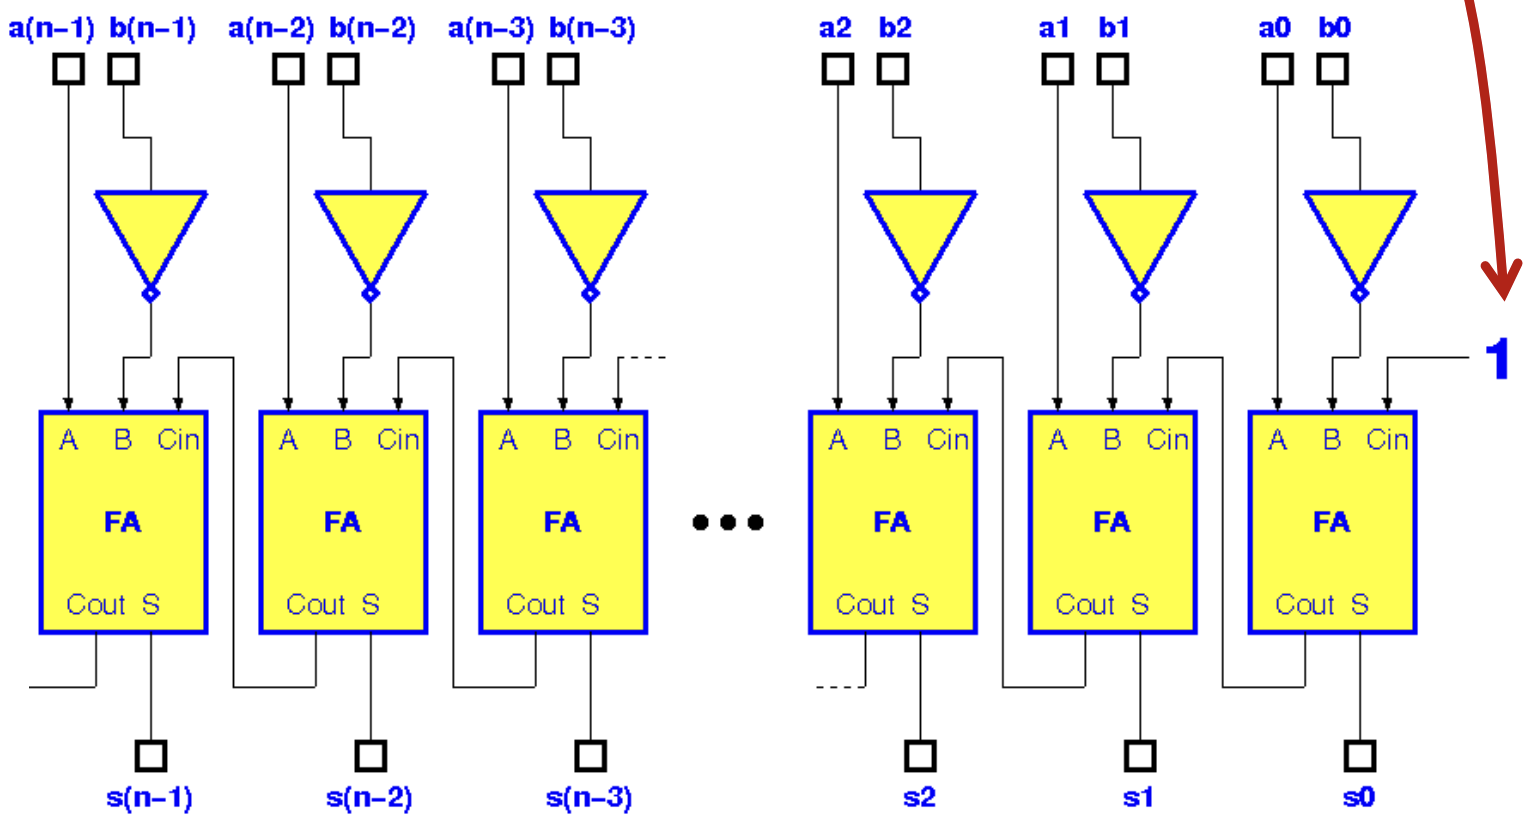
\includegraphics[width=0.65\textwidth]{chapters/chapter1e/images/substractor.png}
\end{center}

\subsection{Two's Complement Add/Subtract Unit}
This circuit performs both addition and subtraction using two's complement arithmetic. The operation is selected based on the control input signal for subtraction. The unit consists of several key components:

\begin{itemize}
    \item[-] \textbf{Input Inversion:} Each bit of the subtrahend $B$ is passed through a XOR gate controlled by the `subtract` signal. When the `subtract` signal is high (logic 1), the bits of $B$ are inverted to form the two's complement of $B$, effectively switching the operation to subtraction.
    
    \item[-] \textbf{Addition:} The ripple-carry adder, represented by the ADDER block, performs binary addition of the bits from $A$ and $B$. The carry-in ($Cin$) to the least significant bit is used to add 1 when performing subtraction, completing the two's complement process.
    
    \item[-] \textbf{Overflow Detection:} The overflow generator block detects if the result of the addition/subtraction operation has exceeded the range representable by the fixed number of bits. The `overflow` output is asserted in such cases.
    
    \item[-] \textbf{Output:} The result of the operation is provided as the sum output ($S$), representing either the sum $A + B$ or the result of $A - B$, depending on the control signal.
\end{itemize}

\begin{center}
    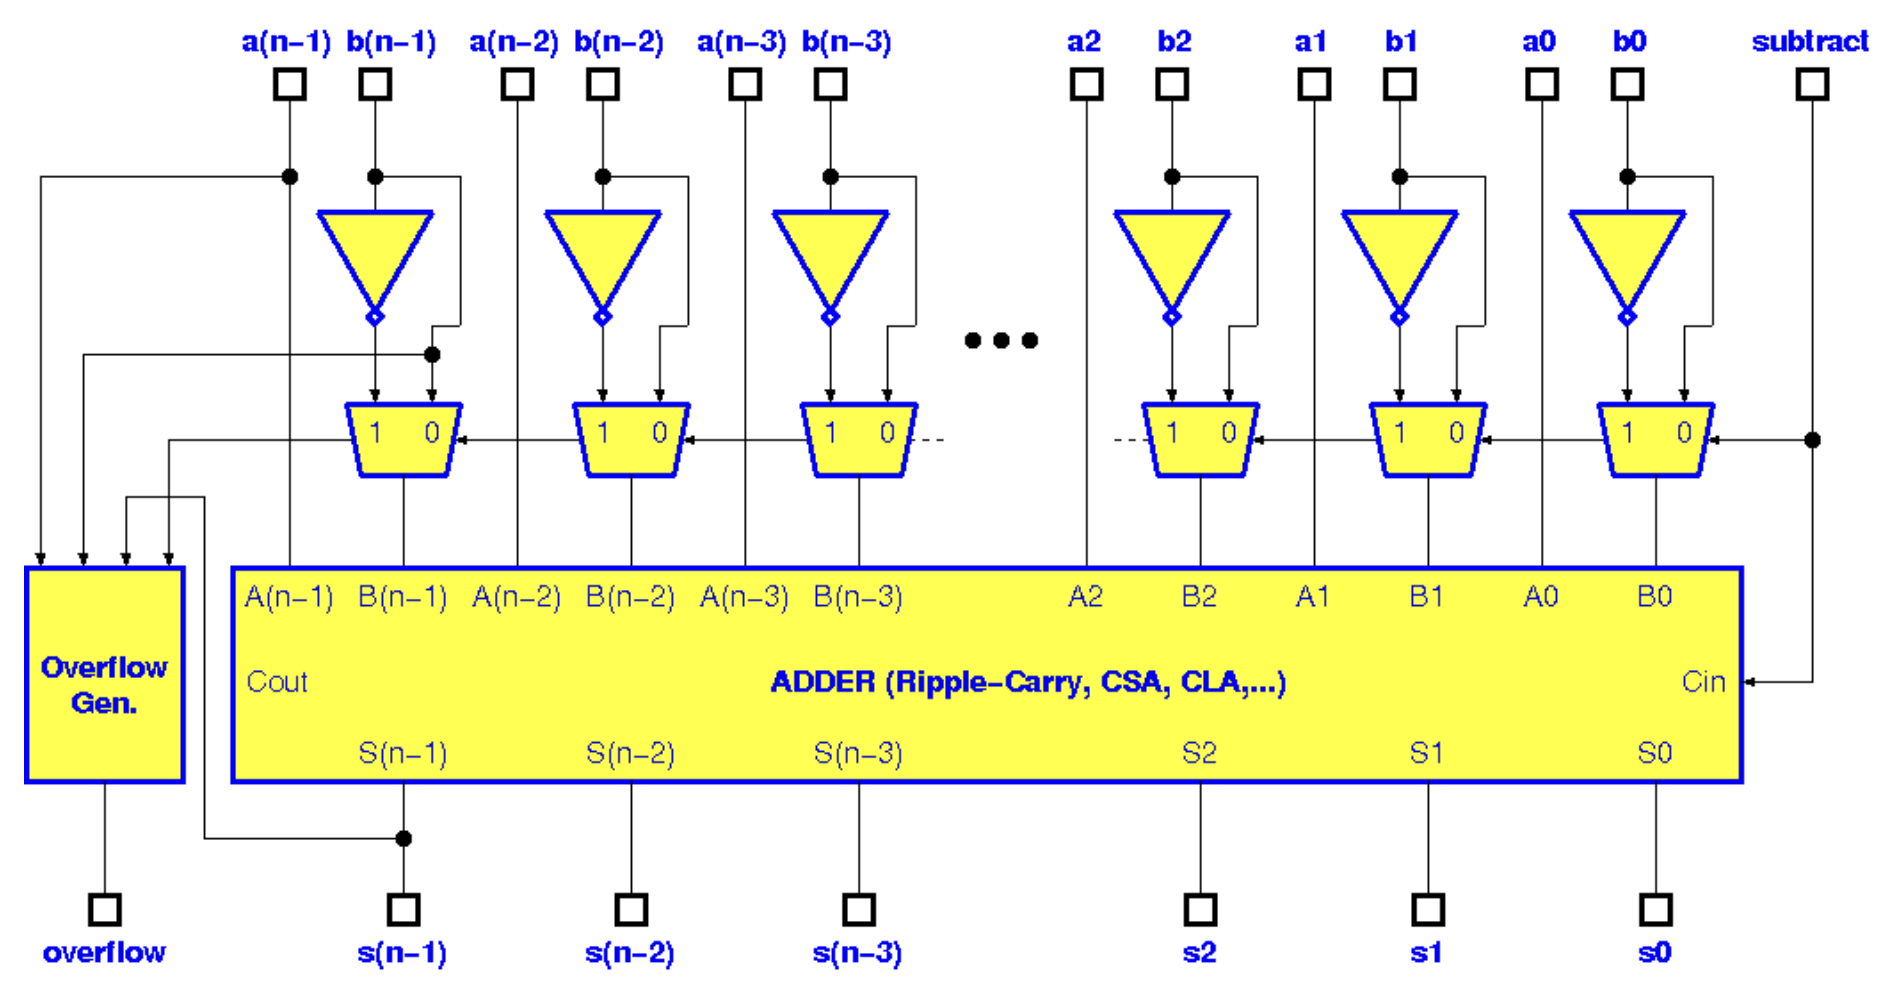
\includegraphics[width=0.65\textwidth]{chapters/chapter1e/images/adder_substractor.png}
\end{center}


\section{Bounds Check Optimization}
\textit{Very, very, very useful.}
When working with signed integers (e.g., array indices), a common task is to ensure that the index remains within a valid range, typically \(0 \leq t0 < N\), where \(N\) is some predefined boundary. \\
This can be achieved efficiently using a single branch check that combines both lower and upper bound constraints. \\
\vspace*{7px}
\textbf{Single Branch Bound Check} \\
\vspace*{3px}
The instruction \texttt{bgeu} (branch if greater than or equal, unsigned) can perform two checks at once:
\[
\texttt{bgeu}\ t0, t1, \texttt{out\_of\_bound}
\]
Here, \(t0\) is the signed number to be checked, and \(t1 = N\) is the boundary. \\
\vspace*{7px}
\textbf{Explanation} \\
\begin{itemize}
    \item[-] If \(t0 \geq 0\), the behavior of \texttt{bgeu} mimics that of \texttt{bge} (branch if greater than or equal) for signed integers, thus effectively performing an upper bound check.
    \item[-] If \(t0 < 0\), since the comparison is unsigned, \(t0\) will appear as a very large positive value, hence automatically triggering the out-of-bound case.
\end{itemize}

This approach efficiently checks both the lower and upper bounds in one instruction, streamlining the bounds checking process.

\section{Floating Point Representation}

Floating point numbers are widely used in computing to represent real numbers in a way that supports a wide dynamic range. \\
\vspace*{5px}
They are composed of a \textit{significand} (or \textit{mantissa}) and an \textit{exponent} of the base. This representation allows for the approximation of very large and very small values, similar to the way scientific notation is used in everyday practices.\\
\vspace*{5px}
\textbf{Such as}
\begin{align*}
    0.18 \ \mu\text{m} & \quad \rightarrow \quad 0.18 \cdot 10^{-6} \ \text{m} \quad \rightarrow \quad 1.8 \cdot 10^{-7} \ \text{m} \\
    75 \ \text{km} & \quad \rightarrow \quad 75 \cdot 10^{3} \ \text{m} \quad \rightarrow \quad 7.5 \cdot 10^{4} \ \text{m}
\end{align*}


In floating point representation, a number \( X \) is expressed as:
\[
X = (-1)^s \cdot \left(\sum_{i=0}^{n-1} a_i \cdot 2^i \right) \cdot 2^{\left( - e_{m-1} 2^{m-1} + \sum_{j=0}^{m-2} e_j 2^j \right)}
\]
where:
\begin{itemize}
    \item[-] \( s \) is the sign bit,
    \item[-] \( a_i \) represents the bits of the significand (in sign-and-magnitude form),
    \item[-] \( e_j \) represents the bits of the exponent (in 2's complement form).
\end{itemize}

\subsubsection{Properties of Floating Point Numbers}
\begin{itemize}
    \item[-] \textbf{Large dynamic range}, but \textit{variable accuracy}.
    \item[-] Numbers are \textbf{redundant} unless \textit{normalized}.
    \item[-] Floating point operations are \textbf{not associative}, unlike real numbers.
    \item[-] Exponents are typically stored in a \textbf{biased signed representation}, making zero easier to represent and simplifying comparisons in hardware.
    \item[-] The \textbf{mantissa} (significand) is usually normalized such that \(1 \leq m < 2\), with a \textit{hidden bit} to store the leading 1.
\end{itemize}

\subsubsection{Standardization and Hardware Support}
Floating point representation is standardized by the IEEE 754 standard, which is widely adopted in modern computing systems:
\begin{itemize}
    \item[-] \textbf{x86/x64} architectures have supported floating point operations through SSE/AVX extensions since 1999.
    \item[-] \textbf{RISC-V} also includes support for floating point through ISA extensions.
\end{itemize}

\subsubsection{Example: Decimal to IEEE 754 Simple Precision (32 Bits) Conversion}
Convert \( -7.75 \) to IEEE 754 single-precision:

\begin{minipage}[t]{0.45\textwidth}
\vspace*{5px}
\textbf{Step 1: Sign Bit (1 Bit)}\\  
\vspace*{5px}
\( s = 1 \) (negative number). \\
\vspace*{5px} 
\textbf{Step 2: Binary Conversion}\\  
\vspace*{5px}
\( 7_{10} = 111_2 \), \( 0.75_{10} = 0.11_2 \), so \( 7.75_{10} = 111.11_2 \). \\
\textbf{Step 3: Normalize}\\
\vspace*{5px}  
\( 111.11_2 = 1.1111_2 \times 2^2 \). \\
\vspace*{5px}
\textbf{Step 4: Exponent (8 Bits)}\\
\vspace*{5px}  
\( E = 2 + 127 = 129 \), \( 129_{10} = 10000001_2 \).
\end{minipage}
\hfill
\vline
\hfill
\begin{minipage}[t]{0.45\textwidth}

\textbf{Step 5: Mantissa (23 Bits)}\\
\vspace*{3px}  
\begin{justify}
    Take the fractional part after the leading 1 and pad with zeros to make 23 bits:
\end{justify} 
\( 1111 \ 0000 \ 0000 \ 0000 \ 0000 \ 000 \) \\
(fractional part after the leading 1). \\
\vspace*{3px}
\textbf{Step 6: IEEE 754 Representation}\\
\vspace*{3px}  
\[
\boxed{
  \underbrace{1}_{\text{Sign bit}} \ 
  \underbrace{10000001}_{\text{Exponent bits}} \ 
  \underbrace{1111 \ 0000 \ 0000 \ 0000 \ 0000 \ 000}_{\text{Mantissa}}
}
\]
\end{minipage}

\subsection{Sign-and-Magnitude Addition}

In this exercise, we aim to write a function in RISC-V assembler to sum two 32-bit signed numbers represented in sign-and-magnitude (S\&M) format. The result should also be produced in the sign-and-magnitude format.

\begin{itemize}
    \item[-] The two operands are stored in registers \texttt{a0} and \texttt{a1} on entry.
    \item[-] The result should be placed in register \texttt{a0}.
    \item[-] Overflow cases should be ignored.
\end{itemize}

\begin{assembly}
# Load the operands from a0 and a1
# Mask the sign bits
andi t0, a0, 0x7FFFFFFF   # Extract magnitude of a0
andi t1, a1, 0x7FFFFFFF   # Extract magnitude of a1

# Extract the signs (MSB) of both operands
srai t2, a0, 31           # Sign of a0
srai t3, a1, 31           # Sign of a1

# Compare the signs
beq t2, t3, same_sign     # If signs are equal, sum the magnitudes
sub t0, t0, t1            # If signs differ, subtract the magnitudes
j check_result            # Jump to check the result

same_sign:
    add t0, t0, t1            # Add magnitudes if signs are the same

check_result:
    # Restore the sign in the result
    slli t0, t2, 31           # Shift the sign bit into position
    or a0, t0, t1             # Combine sign and magnitude into a0
\end{assembly}














